\chapter{Literature Review}
\label{chapter:litRev}
A number of reseachers have proposed various ideas for implementing an 
FPGA based LU solver. Theme methods varies largely with the degree of parallelism 
extracted from the problem and scheduling methods. \\

Kapre \cite{Kapre} \textit{Kapre} (Figure \ref{fig:Into:kapre}) has proposed an FPGA accelerator for parallelizing
the sparse matrix phase of the open-source Spice3f5 circuit simulator. The acceleration
has been achieved by utilizing the symbolic analysis step of the KLU solver to generate
the data flow graph. This graph is then mapped to the network of processing elements 
connected in Mesh grid. The mesh grid approach provides better scalability to the 
architecture. Also the hardware can be utilized for targeting other task graph
based problems which can be scheduled statically. 

../ReviewLit/
\begin{figure}[H]
    \centering
    \begin{subfigure}[b]{0.5\textwidth}
        \centering
        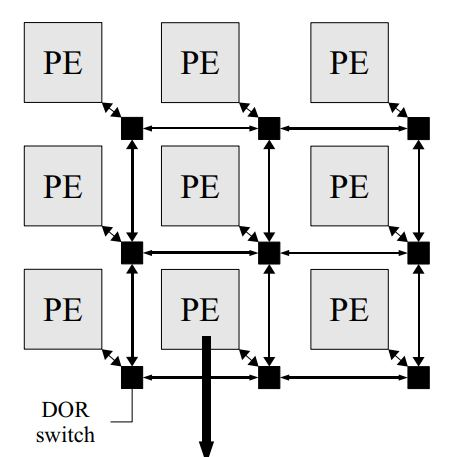
\includegraphics[width = 0.95\linewidth]{./ReviewLit/kapreArch1.JPG}
        \caption{NOC Configuration}
        \label{fig:Intro:KapreNOC}
    \end{subfigure}%
    \begin{subfigure}[b]{0.5\textwidth}
        \centering
        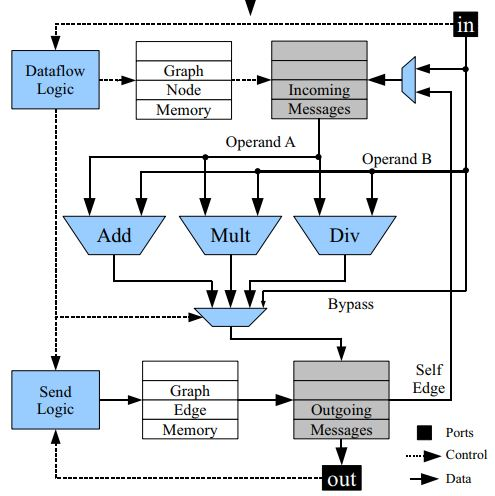
\includegraphics[width = 0.95\linewidth]{./ReviewLit/kapreArch2.JPG}
        \caption{Structure of Processing Element}
        \label{fig:Intro:KaprePE}
    \end{subfigure}
    \caption{NOC based hardware configuration (in \cite{Kapre})}
    \label{fig:Into:kapre}
\end{figure}

In \cite{WuWei}, \textit{Wu and Wei} have utilized the Gilbert-Peierls's algorithm 
to perform symbolic analysis to extract coarse-grain parallelism 
by tearing the matrices into small diagonal sub-problems. These sub-matrices are 
solved parallelly using an FPGA based shared-memory multiprocessor architecture 
called MPoPc. Each node consists of an Altera Nios processor attached to signle-precision
floating point unit.  Reported acceleration are impressive but the benchmark matrices 
are smaller and results were not compared to 
previous FPGA implementations. \\
More recently, \textit{Tarek Nechma and Mark Zwolinski} \cite{Nechma} have presented an approach to 
leverage medium-grain parallelism for LU decomposition based on the column
based parallelism presented bt the Gilbert-Peierls Algorithm. The architecture 
prepares a column execution schedule using the symbolic analysis and maps the
computation of each column to processing element consisting a MAC unit, divider unit
and BRAM. Individual column operations are scheduled using ASAP method. The columns 
are loaded from the main memory with the help of column buffers which is similar to
the DMA engine. Each PE computes the column and then sends updates to the main memory. 
The average reported speedup over KLU is around 9x. However this does not include 
the average time spent on preprocessing in around 36x the factorization time.


\begin{figure}
    \centering
    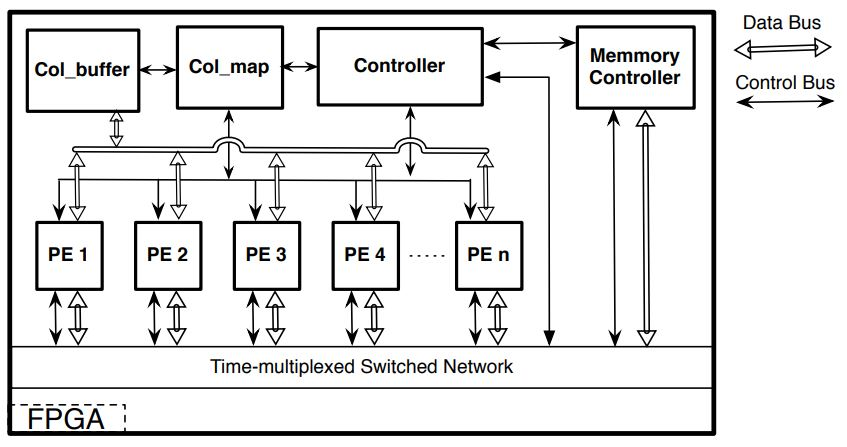
\includegraphics[width = 0.9\linewidth]{./ReviewLit/nechmasArchitecture.JPG}
    \caption{Hardware Architecture used by Nechma \cite{Nechma}}
    \label{fig:Intro:nechma}
\end{figure}


The method used in this report is based on the approach similar to the Nechma's \cite{Nechma}. 
Our scheduler is geared to leverage the fine-grain parallelism using the set of 
deeply pipelined processing elements and low latency block RAMs available in FPGAs. 